\chapter{Anwendung}

Um mithilfe der Playbooks aus diesem Projekt einen Kubernetes-Cluster einzurichten, müssen Material und Infrastruktur vorbereitet werden.
Anschließend werden die SD-Karten einzeln mit Raspbian beschrieben und mit dem Playbook \texttt{local-""raspbian} für den Headless-Betrieb konfiguriert.
Sobald alle Raspberry Pis online sind, wird Kubernetes mit dem Playbook \texttt{kubernetes} aufgesetzt.

% https://www.draw.io/?title=hm#R7VnLcpswFP0alu4YBDZe1uTRNmnr1M1rKZsbUCyQI4Qf%2BfoKEJYxncSJhzDudONBB12Je67OkZQYyItW5xzPw%2B%2FMB2pYXX9loBPDsgauKX8zYF0AjmMXQMCJX0CmBsbkGRTYVWhKfEgqHQVjVJB5FZyyOIapqGCYc7asdntgtDrrHAdQA8ZTTOvoLfFFWKCu1df4FyBBWM5s9gbFmwiXnVUmSYh9ttyC0KmBPM6YKJ6ilQc0467k5fbr%2BpZeznrn366SJ3w9vPj946ZTDHb2lpBNChxi8e6hf94n%2BPrz1ew56EcL07UHN1d3HZXrAtNU8aVyFeuSQPAln6rJuAhZwGJMTzU65CyNfcim6cqW7nPJ2FyCpgQfQYi1Whw4FUxCoYioelvMmU20U7NXElb9EpbyKbyQJVLrDvMAxAv93E1VpRqARSD4WsZxoFiQRfXjsFqXwaaf5l4%2BKPrfUApUK8UvnMwnBMfZsqc4CSGuFUdTn%2FG4DImA8RznZCylnP9G8wK4gNU7iK4To0axlUCUQ5ilYJZab2ZpB%2BGW1lC3KSpRG6sYVkTcZeGfHNW633pzslIj54112YhlvltBWfN%2B%2B50Oy1tlXNOKcfdUDLLalIxbk8yI4vWEsZlh9aj87uGEy6dA5IwVyAOTBElBYZV%2F7ynNDHzoSUoIyO7dH7DUcBlOmdxSOnyjyGIw%2BdXFeNU59Kw4TR4MDxlDL%2BTHIt%2F%2BnvJ1mpKvOfgv38Pka%2B6746E25bs5WH1sndup2aulMA%2BthQodMZI7XOkR%2Faq8rR3VFt%2BlgraPjzvjDJzKMLt7d7Eka8Pk62KTzAGWUD8djU86F1h6YRaaHZEuSZyuOiMvKxKJKQRH4re9Pe3Wbuy05LRpt%2BaW2WrrfZvdmi3bLbL2tVu7Tb8tP%2FMFEY1IRT6ZmORxShyJlDbt1o4uqFejOAZSZ%2B8jzzPvEZhZ2Rm12toSmP1Rm%2Bhh1a9fSB7x8ZnrkdYe9VutvV03VxL72VSUQm6tifwNIPdTmcdZ3VJDFk3S5HU7xZQEsXyeSobllbU5f7W6VYPd11%2Fdxvy1X2O5sSv%2FLJ0Aj0FA8k9d95FTranjNLZnyqb%2B83hxFdD%2FY0CnfwA%3D
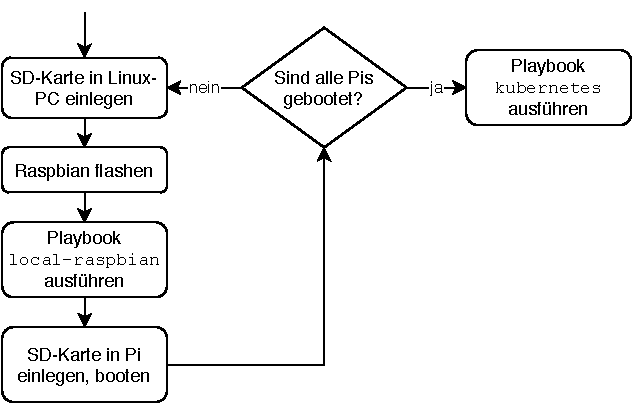
\includegraphics[width=\textwidth]{img/anwendung.pdf}

\section{Vorbereitung}
Zum erfolgreichen Ausführen dieser Anleitung müssen folgende Voraussetzungen erfüllt sein:

\begin{itemize}
    \item \textbf{Raspberry Pis} in beliebiger Anzahl und ebenso viele Speicherkarten und Netzteile stehen bereit.
    \item \textbf{Ein Linux-Rechner} steht bereit, um die Speicherkarten zu flashen und die Ansible-Playbooks auszuführen. Dafür sind Balena Etcher\footnote{\url{https://www.balena.io/etcher/}} und Ansible\footnote{z. B. \texttt{apt install ansible}} installiert, das Git-Repo zu diesem Projekt mit den Verzeichnissen \texttt{inventory} und \texttt{playbook} ist ausgecheckt und ein Image von Raspbian Lite\footnote{\url{https://downloads.raspberrypi.org/raspbian_lite/images/raspbian_lite-2020-02-14/2020-02-13-raspbian-buster-lite.zip}} ist heruntergeladen.
    \item \textbf{Ein Terminal} mit \texttt{playbook} als Current Working Directory ist geöffnet.
    \item \textbf{Ein WiFi-Access Point} mit Internetzugriff ist in Betrieb. Seine Einstellungen (IP, SSID, WPA2-Key) entsprechen den Angaben in den Dateien \texttt{inventory/""group\_vars/""all.yaml} und \texttt{playbook/""local-""raspbian.yaml}. Der zuvor erwähnte Rechner ist mit dem Access Point verbunden.
    \item \textbf{Die Inventory-Datei} \texttt{inventory/""k8s-cluster.yaml} bildet den derzeitigen Cluster ab -- enthält also keine Einträge unter \texttt{hosts}, falls ein neuer Cluster eingerichtet werden soll:

        \begin{lstlisting}
nodes:
  hosts:
        \end{lstlisting}
        \caption{Leere Inventory-Datei}
\end{itemize}

Die benötigte Zeit für die gesamte Einrichtung beträgt ca. 10 Minuten pro Raspberry Pi plus ca. 30 Minuten für den gesamten Cluster.

\section{Raspbian installieren}
Die Schritte in diesem Abschnitt müssen für jeden Raspberry Pi einzeln durchgeführt werden.

\begin{enumerate}
    \item Speicherkarte in den Linux-Rechner einlegen.
    \item Raspbian-Image mit Balena Etcher auf die Speicherkarte flashen.
    \item Raspbian-Playbook ausführen:
        \begin{lstlisting}
ansible-playbook -i ../inventory/k8s-cluster.yaml local-raspbian.yaml
        \end{lstlisting}
        \caption{CLI-Befehl zur Ausführung des Raspbian-Playbooks}
    \item Speicherkarte in den Raspberry Pi einsetzen und booten.
\end{enumerate}

\section{Cluster aufsetzen}

Wenn alle Raspberry Pis gestartet sind, wird die Installation mit dem Kubernetes-Playbook fortgesetzt:
\begin{lstlisting}
ansible-playbook -i ../inventory/k8s-cluster.yaml kubernetes.yaml
\end{lstlisting}
\caption{CLI-Befehl zur Ausführung des Raspbian-Playbooks}

Der Kubernetes-Cluster ist anschließend einsatzbereit.

\section{Weitere Nodes hinzufügen}

Sollen zu einem fertigen Cluster weitere Nodes hinzugefügt werden, kann auch dafür diese Anleitung verwendet werden.
Die Inventory-Datei darf dann nicht leer sein, sondern muss die bereits vorhandenen Nodes enthalten.
